%%%%%%%%%%%%%%%%%%%%%%%%%%%%%%%%%%%%%%%%%
% Beamer Presentation
% LaTeX Template
% Version 1.0 (10/11/12)
%
% This template has been downloaded from:
% http://www.LaTeXTemplates.com
%
% License:
% CC BY-NC-SA 3.0 (http://creativecommons.org/licenses/by-nc-sa/3.0/)
%
%%%%%%%%%%%%%%%%%%%%%%%%%%%%%%%%%%%%%%%%%

%----------------------------------------------------------------------------------------
%	PACKAGES AND THEMES
%----------------------------------------------------------------------------------------

\documentclass{beamer}

\mode<presentation> {

% The Beamer class comes with a number of default slide themes
% which change the colors and layouts of slides. Below this is a list
% of all the themes, uncomment each in turn to see what they look like.

%\usetheme{default}
%\usetheme{AnnArbor}
%\usetheme{Antibes}
%\usetheme{Bergen}
%\usetheme{Berkeley}
%\usetheme{Berlin}
%\usetheme{Boadilla}
%\usetheme{CambridgeUS}
%\usetheme{Copenhagen}
%\usetheme{Darmstadt}
%\usetheme{Dresden}
%\usetheme{Frankfurt}
%\usetheme{Goettingen}
%\usetheme{Hannover}
%\usetheme{Ilmenau}
%\usetheme{JuanLesPins}
%\usetheme{Luebeck}
%\usetheme{Madrid}
%\usetheme{Malmoe}
%\usetheme{Marburg}
%\usetheme{Montpellier}
%\usetheme{PaloAlto}
%\usetheme{Pittsburgh}
\usetheme{Rochester}
%\usetheme{Singapore}
%\usetheme{Szeged}
%\usetheme{Warsaw}

% As well as themes, the Beamer class has a number of color themes
% for any slide theme. Uncomment each of these in turn to see how it
% changes the colors of your current slide theme.

%\usecolortheme{albatross}
%\usecolortheme{beaver}
%\usecolortheme{beetle}
%\usecolortheme{crane}
%\usecolortheme{dolphin}
%\usecolortheme{dove}
%\usecolortheme{fly}
%\usecolortheme{lily}
%\usecolortheme{orchid}
%\usecolortheme{rose}
%\usecolortheme{seagull}
%\usecolortheme{seahorse}
%\usecolortheme{whale}
%\usecolortheme{wolverine}

%\setbeamertemplate{footline} % To remove the footer line in all slides uncomment this line
%\setbeamertemplate{footline}[page number] % To replace the footer line in all slides with a simple slide count uncomment this line

%\setbeamertemplate{navigation symbols}{} % To remove the navigation symbols from the bottom of all slides uncomment this line
}

\usepackage{graphicx} % Allows including images
\usepackage{booktabs} % Allows the use of \toprule, \midrule and \bottomrule in tables

%----------------------------------------------------------------------------------------
%	TITLE PAGE
%----------------------------------------------------------------------------------------

\title[Lisp machines]{Lisp Machines and the Analysis of Their High-Level Language Computer Architecture} % The short title appears at the bottom of every slide, the full title is only on the title page

\author{Dominic Dabish and Evan Bradley} % Your name
\institute[OU] % Your institution as it will appear on the bottom of every slide, may be shorthand to save space
{
Oakland University \\ % Your institution for the title page
\medskip
\textit{\{dadabish, edbradley\}@oakland.edu} % Your email address
}
\date{April 2016} % Date, can be changed to a custom date

\begin{document}

\begin{frame}
\titlepage % Print the title page as the first slide
\end{frame}

\begin{frame}
\frametitle{Overview} % Table of contents slide, comment this block out to remove it
\tableofcontents % Throughout your presentation, if you choose to use \section{} and \subsection{} commands, these will automatically be printed on this slide as an overview of your presentation
\end{frame}

%----------------------------------------------------------------------------------------
%	PRESENTATION SLIDES
%----------------------------------------------------------------------------------------

%------------------------------------------------
\section{History of Lisp machines} % Sections can be created in order to organize your presentation into discrete blocks, all sections and subsections are automatically printed in the table of contents as an overview of the talk
%------------------------------------------------

%\subsection{Test} % A subsection can be created just before a set of slides with a common theme to further break down your presentation into chunks

%------------------------------------------------

\begin{frame}
	\frametitle{Early history of Lisp}
	\begin{itemize}
		\item Lambda Calculus introduced in 1930s by Alonzo Church
		\newline
		\item Fortran in 1957
		\newline
		\item No programming languages optimized for artificial intelligence
		\newline
		\item Lisp designed in 1958 by John McCarthy
		\newline
		\item Lisp code implemented on IBM 170 months after
		\newline
	\end{itemize}
\end{frame}

\begin{frame}
	\frametitle{Lisp machines}
	\begin{columns}[c] % The "c" option specifies centered vertical alignment while the "t" option is used for top vertical alignment
		
		\column{.65\textwidth} % Left column and width
		\begin{itemize}
			\item Lisp machines released in mid-1970s, became popular in 1980s
			\item Manufactured by Symbolics, Lisp Machines, Inc., Xerox, TI
			\item Offered GUIs, advanced programmability, flexibility
			\item Noncompetitive hardware
			\item Eventually became outperformed by general-purpose computers
			\item Vendors went bankrupt in 1990s
		\end{itemize}
		
		\column{.5\textwidth} % Right column and width
		\begin{figure}
		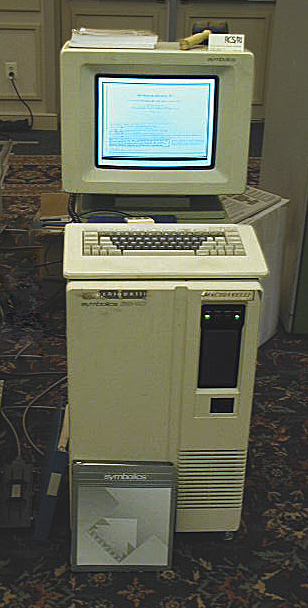
\includegraphics[width=0.6\linewidth]{../img/Symbolics3640}
		\end{figure}
		
	\end{columns}
\end{frame}


%------------------------------------------------
\section{How Lisp works}
%------------------------------------------------


\begin{frame}[fragile] % Need to use the fragile option when verbatim is used in the slide
	\frametitle{Functions in Lisp}
	
	
	Consider a simple function \texttt{g}, which takes one argument \texttt{x}.
	
	
	\begin{example}[Function in mathematics]
		\begin{verbatim}
		g(x)
		\end{verbatim}
	\end{example}
	
	
	In Lisp, this is written in the following manner:
	
	\begin{example}[Function in Lisp]
		\begin{verbatim}
		(g x)
		\end{verbatim}
	\end{example}
	
\end{frame}

\begin{frame}[fragile] % Need to use the fragile option when verbatim is used in the slide
	\frametitle{Lists}
	
	
	\begin{columns}[c] 
		\column{.6\textwidth} % Left column and width
	Consider a simple array of characters in Java:
	
	\begin{example}[Array in Java]
		\begin{verbatim}
		char[] myArray = ['d', 'o', 'm'];
		\end{verbatim}
	\end{example}
	
	
	In Lisp, we can write the elements as symbols, and our data structure is a \texttt{list}.
	
	\begin{example}[List in Lisp]
		\begin{verbatim}
		'(d o m)
		\end{verbatim}
	\end{example}
	
	\column{.5\textwidth} % Left column and width
	\begin{figure}
		
\includegraphics[width=1.2\linewidth]{../img/chain}
		 
	\end{figure}
	
	
	\end{columns}
	
\end{frame}

\begin{frame}[fragile] % Need to use the fragile option when verbatim is used in the slide
	\frametitle{List-manipulating functions}
	
	\texttt{car} and \texttt{cdr} are primitive operations for lists.
	
	\begin{itemize}
		\item \texttt{car} extracts the first element from the list
		\item \texttt{cdr} extracts the rest of the list
	\end{itemize}
	
	
	\begin{example}[car]
		\begin{verbatim}
		(car '(d o m)) => 'd
		\end{verbatim}
	\end{example}
	
	\begin{example}[cdr]
		\begin{verbatim}
		(cdr '(d o m)) => '(o m)
		\end{verbatim}
	\end{example}
	
\end{frame}

\begin{frame}[fragile]
	\frametitle{Defining a recursive function}
		Let us define a factorial function in Lisp using recursion:\\
		\begin{example}[Factorial function in Lisp]
			\begin{verbatim}
			(defun factorial(n)
			    (if (= n 0)
			        1
			        (* n (factorial (- n 1))
			    )
			)
			\end{verbatim}
		\end{example}
		
\end{frame}

\begin{frame}[fragile]
	\frametitle{Evaluating a recursive function}
	\begin{table}
		Consider the following function call:
		\begin{example}[Factorial function call in Lisp]
			\begin{verbatim}
			(factorial 5)
			\end{verbatim}
		\end{example}
		
		Here is its evaluation path:
		\begin{tabular}{l l l l}
			\toprule
			\textbf{Function call} & \textbf{Evaluation 1} & \textbf{Eval 2} & \textbf{Eval 3}\\
			\midrule
			\texttt{(factorial 5)} &\texttt{(* 5 (factorial 4))} & \texttt{(* 5 24) } & \texttt{120} \\
			\texttt{(factorial 4)} &\texttt{(* 4 (factorial 3))} & \texttt{(* 4 6)  } & \texttt{24} \\
			\texttt{(factorial 3)} &\texttt{(* 3 (factorial 2))} & \texttt{(* 3 2)  } & \texttt{6} \\
			\texttt{(factorial 2)} &\texttt{(* 2 (factorial 1))} & \texttt{(* 2 1)  } & \texttt{2} \\
			\texttt{(factorial 1)} &\texttt{(* 1 (factorial 0))} & \texttt{(* 1 1)  } & \texttt{1} \\
			\bottomrule
		\end{tabular}
		\caption{Complete recursive evaluation}
	\end{table}
\end{frame}


\begin{frame}[fragile]
	\frametitle{Recursive evaluation example explained}

	\begin{columns}[c] % The "c" option specifies centered vertical alignment while the "t" option is used for top vertical alignment
		
		
		\column{.4\textwidth} % Left column and width
		
		Is the argument \texttt{n} is equal to 0 (the base case)?
			\begin{itemize}
				\item \textbf{YES}: the function evaluates to 1 and terminates.
				\item \textbf{NO}: the function will multiply the argument by the factorial with \texttt{n-1} as the argument.\\
			\end{itemize}
		
		
		This creates a chain, and evaluates to the factorial of \texttt{n}.
		
		  
		
		\column{.5\textwidth}
		\begin{figure}
			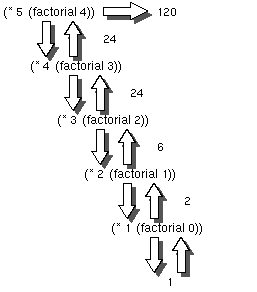
\includegraphics[width=1\linewidth]{../img/factorial}
		\end{figure}

	\end{columns}

\end{frame}


%------------------------------------------------
\section{Problems in Execution}
%------------------------------------------------

%------------------------------------------------
\section{Example processor}
%------------------------------------------------

%------------------------------------------------
\section{Legacy of Lisp machines}
%------------------------------------------------

\begin{frame}
	\frametitle{Legacy of Lisp machines}
		\begin{block}{ }
		LISP is now the second oldest programming language in present widespread use (after FORTRAN). Lisp owes its survival to the fact that its programs are lists, which is actually a disadvantage.\newline\newline-
		John McCarthy, 1979
		\end{block}
		
			\begin{itemize}
				\item Lisp machines dominated in AI (their most popular domain)
				\item Worked very well for domain-specific programming
				\item Introduced new features: Dynamic creation of new objects, dynamically sized-lists, garbage collector
				\item On-the-fly changes - no need to recompile\newline
			\end{itemize}
	
\end{frame}

\begin{frame}
	\frametitle{Legacy of Lisp machines}
	Lisp continues to be a popular tool in
	\begin{itemize}
		\item education
		\item research
		\item general programming\newline
	\end{itemize}
	
		\textit{Lisp and Lisp machines influenced...}
		Haskell, JavaScript, Lua, Mathematica, ML, Nim,  Perl, Python, R, Ruby, Scala, Smalltalk
	
		\begin{columns}[c] % The "c" option specifies centered vertical alignment while the "t" option is used for top vertical alignment
			
			\column{.75\textwidth} 
	
	\textit{Structure \& Interpretation of Computer Programs} is a classic programming textbox,  and uses a Lisp variant to teach programming in universities nationwide, including Oakland University.\newline
	

			
			
			\column{.2\textwidth} 
			\begin{figure}
				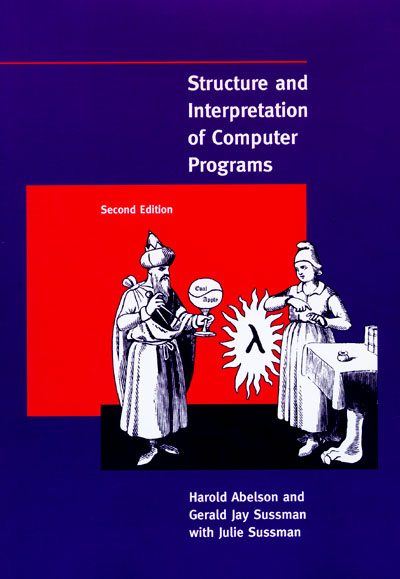
\includegraphics[width=1\linewidth]{../img/SICP}
			\end{figure}
			
		\end{columns}
		
	\end{frame}
	\begin{frame}
		\frametitle{Legacy of Lisp machines}
	
	
	Though Lisp machines are no longer a commercial enterprise,
	
		\begin{itemize}
			\item Lisp has continued interest and usage
			\item Lisp machines serve an important place in history
			\item Many with interest in retro-computing have recreational interest in Lisp machines
		\end{itemize}
		
		... even many years after the last manufacturers ceased to exist
		
		\begin{figure}
			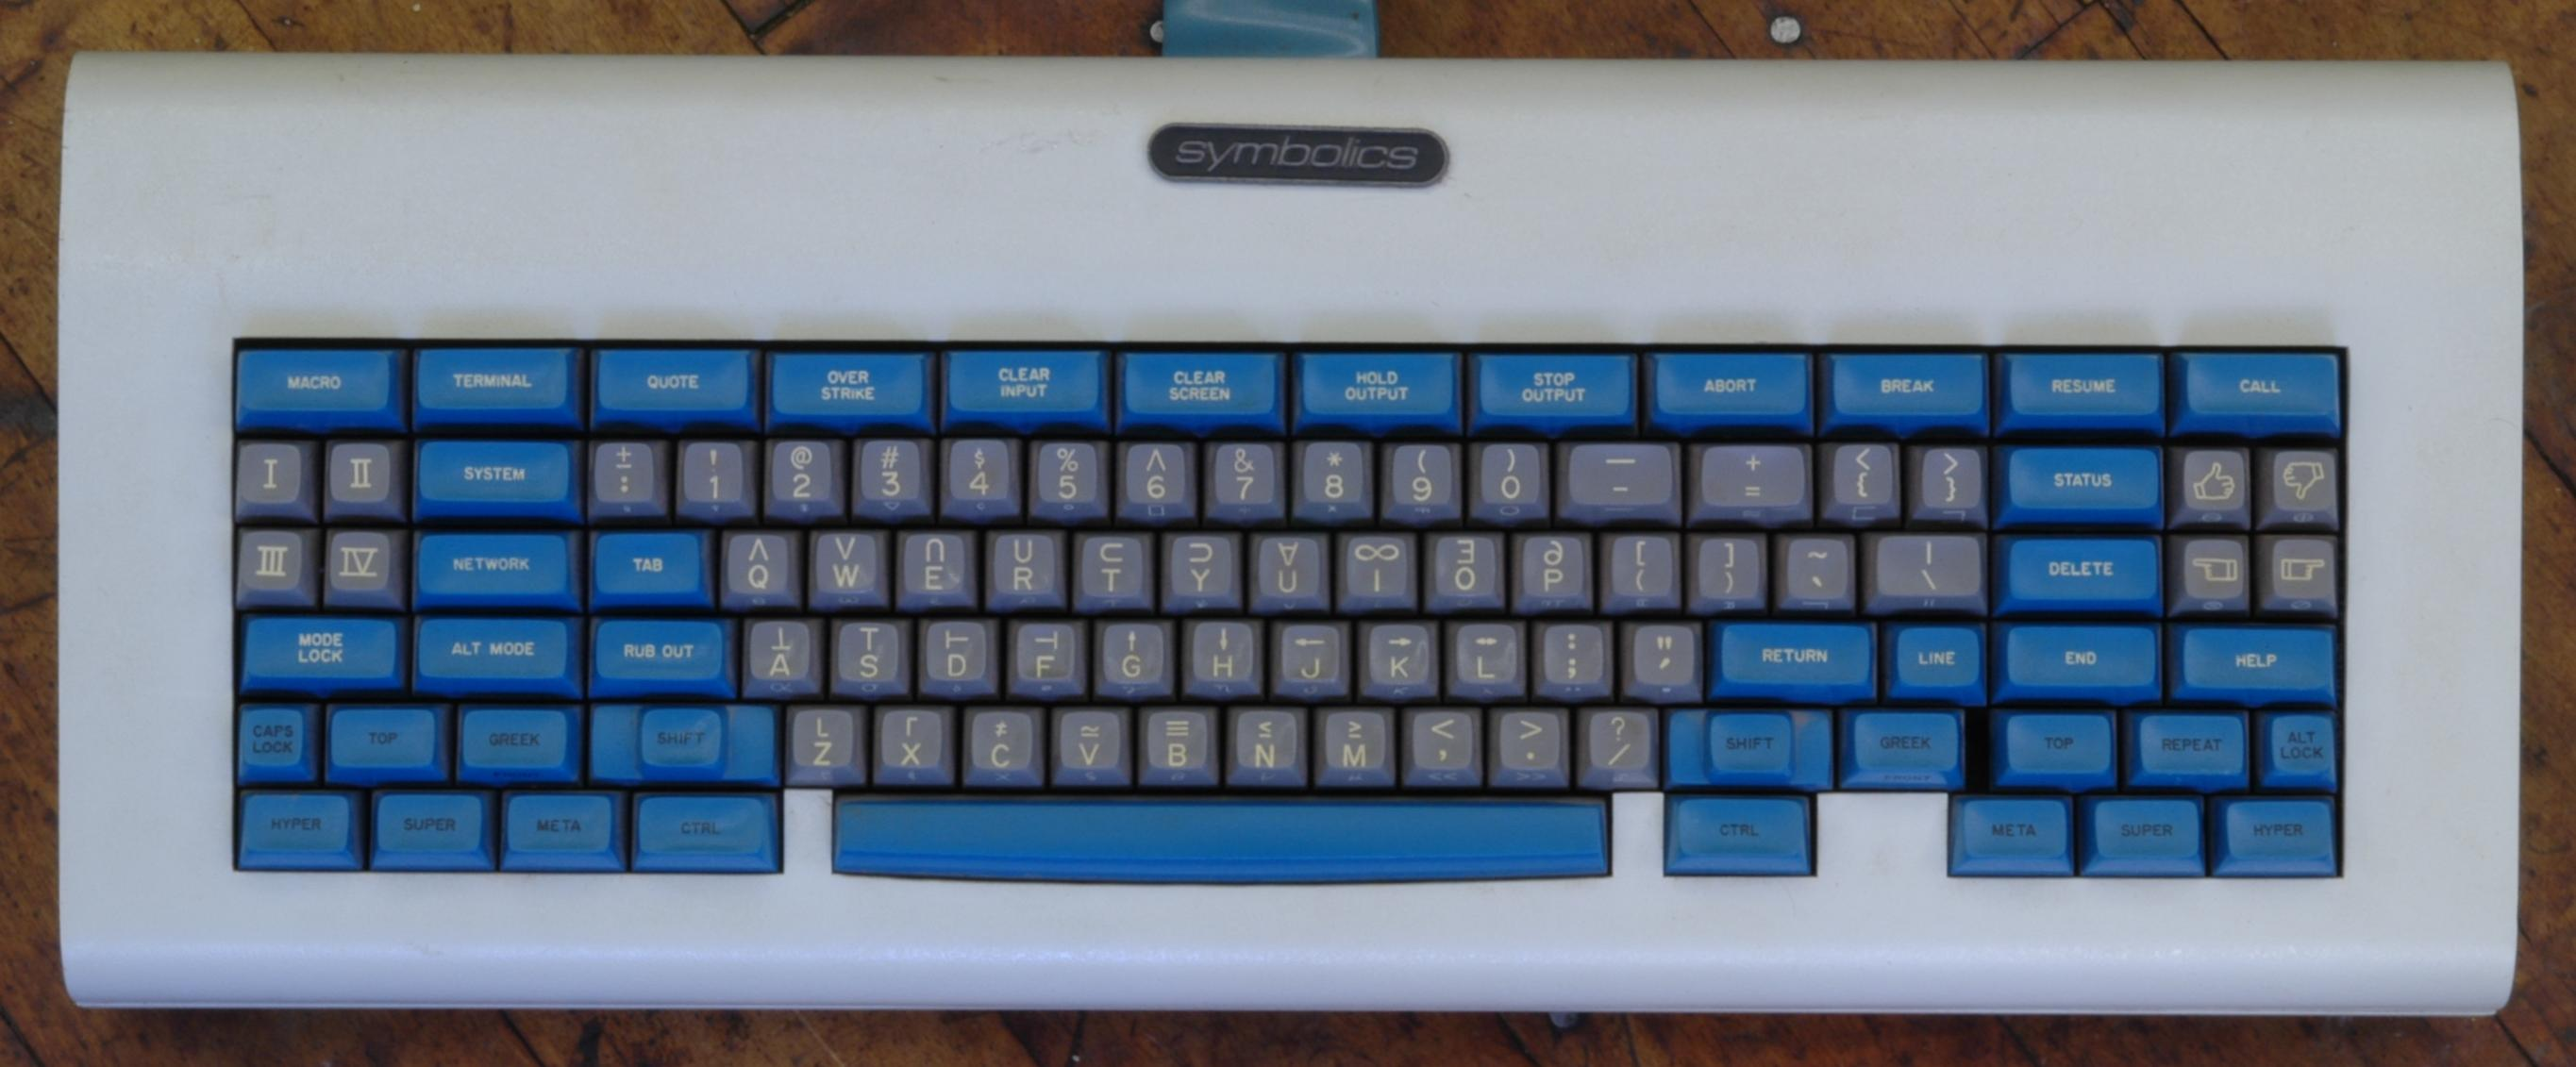
\includegraphics[width=0.6\linewidth]{../img/keyboard}\caption{These \textit{retro keyboards}, that once were used with then-modern Lisp machines, are today collected by hobbyists.}
		\end{figure}
	
\end{frame}


\begin{frame}
	\Huge{\centerline{Thank you!}}
	\Huge{\centerline{ }}
	\Huge{\centerline{Questions?}}
\end{frame}

%----------------------------------------------------------------------------------------

\end{document} 